\let\negmedspace\undefined
\let\negthickspace\undefined
\documentclass[journal]{IEEEtran}
\usepackage[a5paper, margin=10mm, onecolumn]{geometry}
\usepackage{lmodern} % Ensure lmodern is loaded for pdflatex
\usepackage{tfrupee} % Include tfrupee package

\setlength{\headheight}{1cm} % Set the height of the header box
\setlength{\headsep}{0mm}     % Set the distance between the header box and the top of the text

\usepackage{gvv-book}
\usepackage{gvv}
\usepackage{cite}
\usepackage{amsmath,amssymb,amsfonts,amsthm}
\usepackage{algorithmic}
\usepackage{graphicx}
\graphicspath{{./figs/}}
\usepackage{textcomp}
\usepackage{xcolor}
\usepackage{txfonts}
\usepackage{listings}
\usepackage{enumitem}
\usepackage{mathtools}
\usepackage{gensymb}
\usepackage{comment}
\usepackage[breaklinks=true]{hyperref}
\usepackage{tkz-euclide} 
\usepackage{listings}
\usepackage{gvv}                                        
\def\inputGnumericTable{}                    
\usepackage[latin1]{inputenc}                                
\usepackage{color}                                            
\usepackage{array}                                            
\usepackage{longtable}                                       
\usepackage{calc}                            
\usepackage{multirow}                                         
\usepackage{hhline}                                          
\usepackage{ifthen}                                           
\usepackage{lscape}
\usepackage{circuitikz}

\begin{document}
	
	\bibliographystyle{IEEEtran}
\vspace{3cm}

\title{4.11.19}
\author{EE25BTECH11042 - Nipun Dasari}
\maketitle

\renewcommand{\thefigure}{\theenumi}
\renewcommand{\thetable}{\theenumi}
\setlength{\intextsep}{10pt} % Space between text and floats


\numberwithin{equation}{enumi}
\numberwithin{figure}{enumi}
\renewcommand{\thetable}{\theenumi}
	
	\textbf{Question}:\\
	Find the coordinates of the point where the line through the points P\brak{4, 3, 2} and Q\brak{5, 1, 6} crosses the XZ plane. Also find the angle which this line makes with the XZ plane. Solve using matrices and vectors only.
	
	\solution
	
	First, we represent the points P and Q as position vectors.
	\begin{align}
		\vec{p} = \myvec{4 \\ 3 \\ 2}  \text{and}  \vec{q} = \myvec{5 \\ 1 \\ 6}
	\end{align}
	The direction vector, $\vec{d}$
	\begin{align}
		\vec{d} = \vec{q} - \vec{p} = \myvec{5 \\ 1 \\ 6} - \myvec{4 \\ 3 \\ 2} = \myvec{1 \\ -2 \\ 4}
	\end{align}
	Line can be written as $\vec{r} = \vec{p} + \lambda \vec{d}$.
	\begin{align}
		\vec{r} = \myvec{x \\ y \\ z} = \myvec{4 \\ 3 \\ 2} + \lambda \myvec{1 \\ -2 \\ 4} = \myvec{4 + \lambda \\ 3 - 2\lambda \\ 2 + 4\lambda}
	\end{align}
	Equation for x-z plane is
	\begin{align}
		\begin{myvec}{0\\1\\0}\end{myvec}^\top\vec{x}=0
	\end{align}
	On solving for point of intersection
	\begin{align}
		3 - 2\lambda = 0 \implies 2\lambda = 3 \implies \lambda = \frac{3}{2} \label{0.4}
	\end{align}
	By \eqref{0.4}
	\begin{align}
		\vec{r}_{\text{intersection}} = \myvec{4 + \frac{3}{2} \\ 3 - 2(\frac{3}{2}) \\ 2 + 4(\frac{3}{2})} = \myvec{\frac{11}{2} \\ 0 \\ 8}
	\end{align}
	The intersection point is $(\frac{11}{2}, 0, 8)$.
	
	The angle $\theta$ between a line with direction vector $\vec{d}$ and a plane with normal vector $\vec{n}$ is given by:
	\begin{align}
		\sin\brak{\theta}= \frac{|\vec{d}^T\vec{n}|}{\norm{\vec{d}} \norm{\vec{n}}} \label{0.6}
	\end{align}
	The direction vector of the line is $\vec{d} = \myvec{1 \\ -2 \\ 4}$. The normal vector to the XZ plane ($y=0$) is $\vec{n} = \myvec{0 \\ 1 \\ 0}$.
	
	\begin{align}
		\vec{d}^T\vec{n} = \myvec{1 \\ -2 \\ 4}^T\myvec{0 \\ 1 \\ 0} = (1)(0) + (-2)(1) + (4)(0) = -2 \label{0.7}
	\end{align}
	
	\begin{align}
		\norm{\vec{d}} = \sqrt{1^2 + (-2)^2 + 4^2} = \sqrt{1 + 4 + 16} = \sqrt{21} \label{0.8} \\ 
		\norm{\vec{n}} = \sqrt{0^2 + 1^2 + 0^2} = 1 \label{0.9}
	\end{align}
	By \eqref{0.6},\eqref{0.7},\eqref{0.8},\eqref{0.9}
	\begin{align}
		\sin\theta = \frac{|-2|}{\sqrt{21}1} = \frac{2}{\sqrt{21}}
	\end{align}
	Therefore, the angle the line makes with the XZ plane is:
	\begin{align}
		\theta = \arcsin\brak{\frac{2}{\sqrt{21}}}
	\end{align}
	
	\begin{figure}[H]
		\centering
		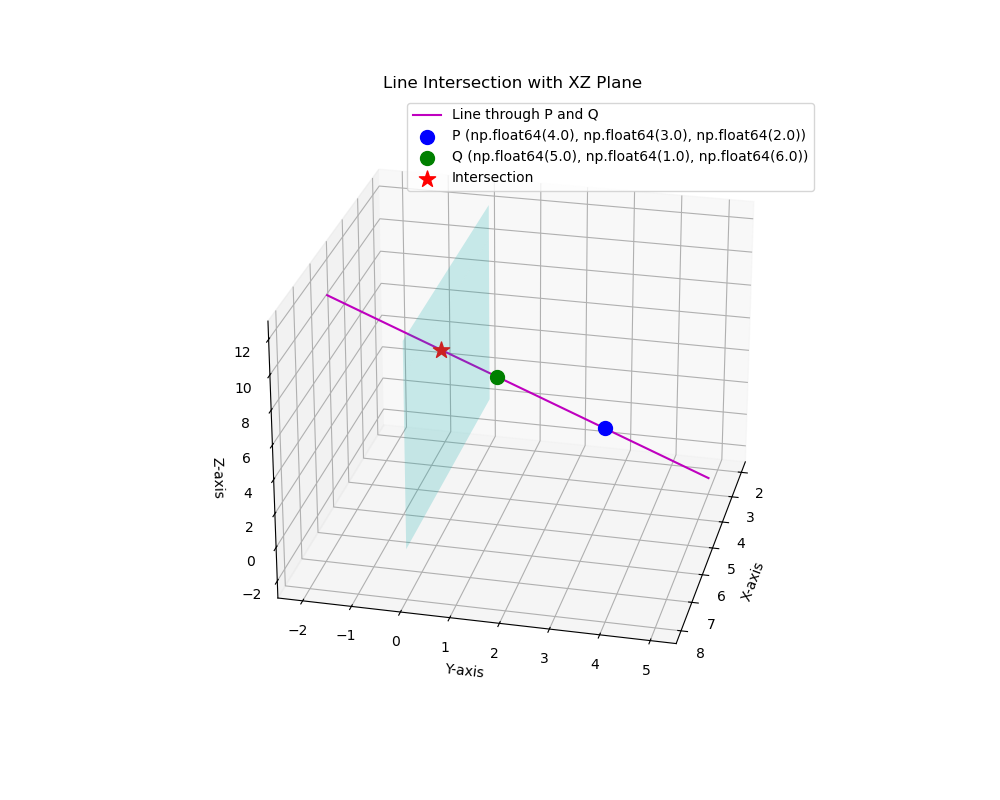
\includegraphics[width = 0.8\columnwidth]{Figure_1.png}
		\caption*{}
		\label{}
	\end{figure}
	
\end{document}